\documentclass[a4paper]{article}

%% Language and font encodings
\usepackage[english]{babel}
% \usepackage[utf8x]{inputenc}
% \usepackage[T1]{fontenc}
% \setmainfont{Noto Serif CJK TC}
\usepackage{fontspec}
\newfontfamily\ZhFont{Droid Sans Fallback}


%% Sets page size and margins
\usepackage[a4paper,top=3cm,bottom=2cm,left=3cm,right=3cm,marginparwidth=1.75cm]{geometry}

%% Useful packages
\usepackage{amsmath}
\usepackage{graphicx}
\usepackage[colorinlistoftodos]{todonotes}
\usepackage[colorlinks=true, allcolors=blue]{hyperref}
\usepackage{algpseudocode,algorithm,algorithmicx}
\usepackage{subcaption}

%new commands
\newcommand*\Let[2]{\State #1 $\gets$ #2}
\newcommand{\prog}[1]{\mbox{{\sc #1}}} 
\newcommand{\fnvar}[1]{\prog{#1}}
\newcommand{\var}[1]{{\it #1}}
\newcommand{\defeq}{\stackrel{\text{def}}{=}}
\newcommand{\name}{{\sc GPO}\xspace}



\title{When RL Meets Evolutionary Computation}
\author{b03902071 \ZhFont 葉奕廷 \\ b03902072 \ZhFont 江廷睿}
\date{}

\begin{document}
\maketitle

\begin{abstract}
Inspired by the recent research which combine reinforcement learning (RL) with evolutionary computation (EC), we explore the connection between genetic algorithm (GA) and RL. Then we further extends the existing algorithms and experiments on games and well-known deceptive problem MK-Trap. We show a more efficient update technique on ES-based RL using existing ES algorithms called CMA-ES and successfully combine GA with Deep Q-learning. 
\end{abstract}

\section{Introduction}

The recent revelation from OpenAI \cite{openes/2017arXiv170303864S} that an evolutionary algorithm can rival modern gradient-based RL approaches in the Mujoco and Atari learning environments is a source of some surprise. We think the most surprising thing is that a simple ES algorithm which does not compute exact gradients can optimize deep neural networks (DNNs) with over a million parameters. There is another paper \cite{DBLP:journals/corr/abs-1711-01012} which shows the combination of policy-based RL and GA can has superior performance over the state-of-the-art policy gradient methods and achieves comparable or higher sample efficiency on Mujoco locomotion tasks. It seems like the popular trend in Deep-RL research field is to combine RL with EC algortihms to fully utilize there 720 cores CPU and speedup training. Thus we are also curious about this combination which looks strange but works well. So we first explain the relation between GA and RL theoretically in Section \ref{sec:GAvsRL}. Secondly we extend algorithms proposed by OpenAI \cite{openes/2017arXiv170303864S} in Section \ref{sec:ESRL} and describe a new algorithm called Genetic Improved Reinforcement Learning (GIRL) to combine value-based RL with genetic algorithm based on \cite{DBLP:journals/corr/abs-1711-01012} in Section \ref{sec:GIRL}. Thirdly we do experiments on the well-known deceptive problem MK-trap and games in OpenAI Gym \cite{gym/2016arXiv160601540B} in Section \ref{sec:ESRL-exp} and Section \ref{sec:GIRL-exp} respectively. Finally we discuss the pro and cons of these algorithms and make the conclusion in Section \ref{sec:conclusion}.

 
\section{Connection between Genetic Algorithm and Reinforcement Learning}
\label{sec:GAvsRL}

Genetic algorithm and reinforcement learning are similar in many aspects. Both genetic algorithm and reinforcement learning can be used to optimize a black function. We can see problems for genetic algorithm as problems for reinforcement algorithm, where the bit string is a sequence of actions our agent needs to decide, while the fitness of the bit string is the total reward of an episode. \par

Specifically, compact genetic algorithm are very similar to the REINFORCE policy optimization algorithm of reinforcement learning \cite{DBLP:journals/ml/Williams92}. In compact genetic algorithm, we generate chromosomes according to some parameters. Then we update the parameters to increase the probability of generating chromosome with high fitness while decrease the probability of generating chromosome with low fitness. That is identical to what REINFORCE algorithm does. The only difference is that REINFORCE updates parameters using the gradient of expected total reward while compact genetic algorithm doesn't. Gradient is definitely not necessarily the best guidance for parameter optimization. Genetic algorithm as well as evolutionary strategy provide powerful tools for such kind of black box function optimization problem. That is one thing we explored as will describe in section \ref{sec:ESRL} and \ref{sec:GIRL}.

It is also interesting to see how reinforcement learning works on MK-trap problem. MK-trap problem was well studied during the our whole semester of genetic algorithm course, and was solved by genetic algorithm with model building. However, to our knowledge, there is no any research about solving MK-trap with reinforcement learning. We thus further experiment on solving MK-trap problem with reinforcement learning. We reformulate the problem, namely the combinatorial problem with $m$ traps of length $k$, into an reinforcement learning "environment" as follow:

\begin{itemize}
\item Episode length: $m \times k$.
\item Action: 0 or 1.
\item Rewards: 0 for steps other than last step, and fitness of the bit string that consists of the made actions for the last step. Here the fitness for each trap is the ratio of 0 in the trap and 2 if all ones. And the fitness of a chromosome is the summation of all traps' fitness.
\item Observation: the agent need to know which bit it is deciding and may need to consider the dependency of the actions it has decided, so for time $t$, the observation is the vector $s \in \{0, 1\}^{2mk}$ where $s_i = 1$ only if the $i$-th action is 0, and $s_{mk + i} = 1$ only if the $i$-th action is 1.
\end{itemize}
The result will be described in section \ref{sec:ESRL} and \ref{sec:GIRL}.

\section{ES-Based Reinforcement Learning}
\label{sec:ESRL}

OpenAI described a general scheme for using Evolution Strategy (ES) to optimize DNN in \cite{openes/2017arXiv170303864S}.
\begin{algorithm}
	\caption{Evolution Strategies for RL \label{alg:ESRL}}
    \begin{algorithmic}[1]
	\Require Learning rate $\alpha_1$, noise standard deviation $\sigma_1$, initial policy parameters $\theta_0$
    \For{$i=0, 1, 2, \dotsc$ }
    	\State sample $\sigma_0 \dotsc \sigma_n \sim \mathcal{N}(0, I)$
        \State Compute returns $F_i = F(\theta_t + \sigma\epsilon_i) for i = 1 \dotsc n$
        \Let{Set $\theta_t+1$}{$\theta_t + \alpha\frac{1}{n\sigma}\sum_{i=1}^{n}F_i\epsilon_i$}
    \EndFor
	\end{algorithmic}
\end{algorithm}
This algorithm repeatedly executes two phases: 1) Stochastically perturbing the parameters of the policy (or we can say that we sample parameters from normal distribution $\mathcal{N}(\mu, \sigma)$) and evaluating the resulting parameters by running an episode in the environment, and 2) Combining the results of these episodes, calculating a stochastic gradient estimate, and updating the parameters. In OpenAI's paper, they use REINFORCE algorithm \cite{Williams:1992:SSG:139611.139614} to update parameters but fix the standard deviation $\sigma$ to $I$ when sampling from normal distribution. However we know the step size control is particularly important and powerful component in ES, so here we extend the algorithm to better utilize the power of ES.

\subsection{PEPG}
Proposed in \cite{PEPG}, we can also use REINFORCE algorithm to update $\sigma$ to better explore parameter space. To be more specific, the update rule of REINFORCE algorithm can be written as $\nabla_\theta J(\theta) \approx \frac{1}{N}\sum_{i=1}^{N}F(z^i)\nabla_\theta \log\pi(z^i, \theta)$, and we can update $\sigma$ by $\nabla_(\sigma_j) \log N(z^i, \mu, \sigma) = \frac{(z^i_j - \mu_j)^2 - \sigma^2_j}{\sigma^3_j}$ where $z^i$ is the sampled solution.

\subsection{CMA-ES}
CMA-ES \cite{Auger:2012:TCE:2330784.2330919} is the well-known and very powerful ES algorithm. Similarly, CMA-ES takes the results from each generation and adjust our step size. Different to PEPG, it will not only adapt for the $\mu$ and $\sigma$ of the normal distribution but calculate the entire covariance matrix of the parameter space.

\subsection{Experiments}
\label{sec:ESRL-exp}

\subsubsection*{LunarLander}
In the environment LunarLander, agent learns to guide a space vehicle from starting point to the landing pad without crashing. If the lander  successfully moves from the top of the screen to landing pad is about 100..140 points. If the lander does not crash and comes to rest, it can get additionally 100 points otherwise -100 points. Some bonus points are for special techniques. LunarLander defines "solving" as getting average reward of 200 over 100 consecutive trials.
We set the population size to 50 and problem size (i.e. parameter number) to 2788, which is equivalent to the DNN with hidden size 64, 32.

We find that the vanilla REINFORCE algorithms can not play this game without proper state preprocessing and time-wasting hyperparameter tuning, so we report Deep Q-learning (DQN) as our baseline. In figure \ref{fig:learning-curve-es-lunarlander}, CMA-ES performs significantly better than the other two algorithms, and to our surprise OpenAI-ES is better than PEPG. We think the reason is that gradient is not a stable way to adjust the exploration step, and in LunarLander such unstable update of the $\sigma$ is hurtful. Because the x-axis of the figure \ref{fig:learning-curve-cma-es-lunarlander} and \ref{fig:learning-curve-dqn-lunearlander} are different (DQN updates according to the environment steps while CMA-ES updates according to generations), we can only say the training of CMA-ES is more stable than DQN and the inference times of fitness function are roughly the same magnitude (DQN runs 3980 episodes to solve this game while CMA-ES sees $80 * 50 * 5$ episodes (generations * population size * trails to evaluate each chromosome). But in the real time CMA-ES is significantly faster than DQN which trains on GeForce GTX 1080 Ti when we parallelize the program properly. So if the input is not the raw pixel (otherwise the input dimension will be too large), CMA-ES is the better choice to use.

\begin{figure}[H]
\centering
\begin{subfigure}{.3\textwidth}
  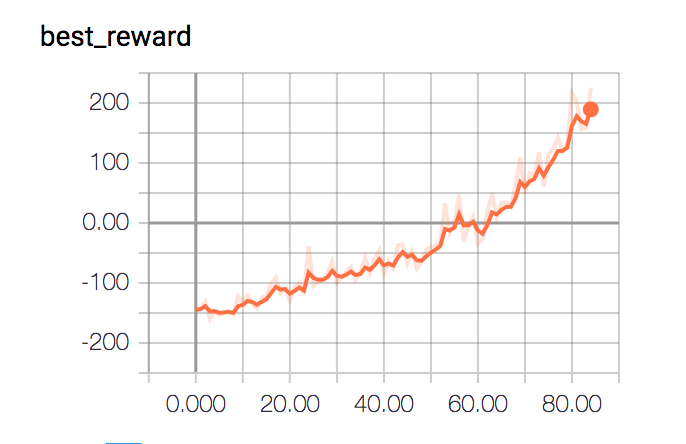
\includegraphics[width=\linewidth]{figures/cma-es-lunarlander.png}
  \caption{Learning Curve of CMA-ES}
  \label{fig:learning-curve-cma-es-lunarlander}
\end{subfigure}
\begin{subfigure}{.3\textwidth}
  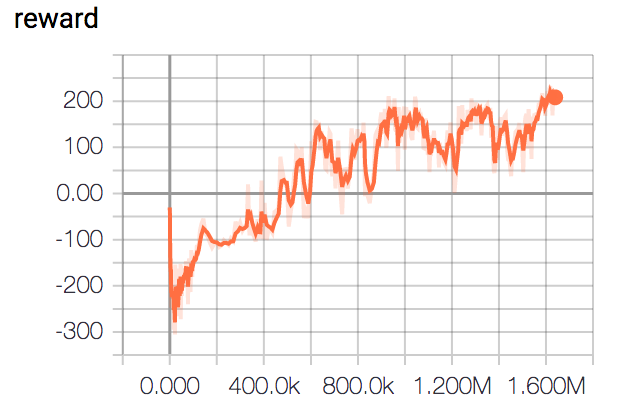
\includegraphics[width=\linewidth]{figures/dqn-lunarlander.png}
  \caption{Learning curve of DQN}
  \label{fig:learning-curve-dqn-lunearlander}
\end{subfigure}
\begin{subfigure}{.3\textwidth}
	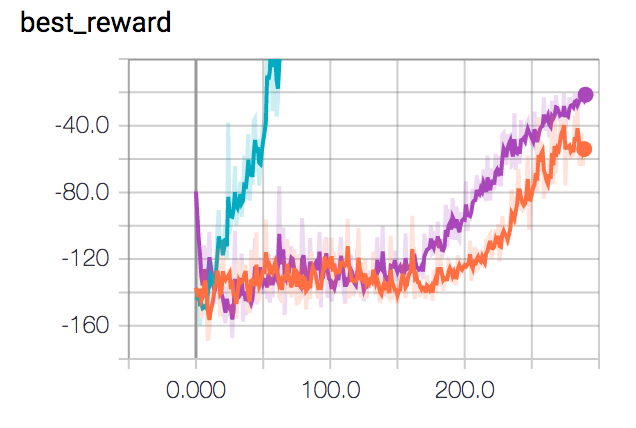
\includegraphics[width=\linewidth]{figures/ES-lunarlander.png}
	\caption{Learning curve of three different ES algorithms. Blue is CMA-ES, purple is OpenAI-ES and orange is PEPG}
	\label{fig:learning-curve-es-lunarlander}
\end{subfigure}
\caption{Learning curve of CMA-ES, OpenAI-ES, PEPG and DQN for environment LunarLander}
\label{fig:learning-curve-cma-es-dqn-compare-lunarlander}
\end{figure}

\subsection*{MK-Trap}

Vanilla REINFORCE and those three ES algorithms can't solve MK-trap problem. We think it is reasonable because there are no exploration nor update techniques in REINFORCE, and no niching in these three ES algorithms. That is why we should do model building and consider niching in GA.

\begin{figure}[H]
\centering
\begin{subfigure}{.45\textwidth}
  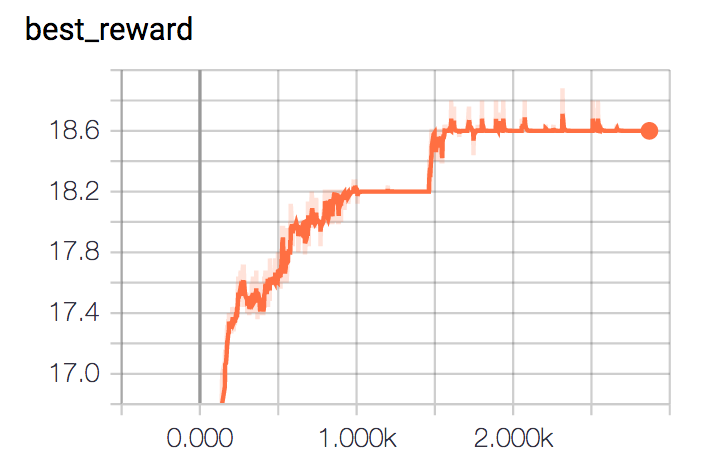
\includegraphics[width=\linewidth]{figures/cmaes-mktrap.png}
  \caption{Learning Curve of CMA-ES}
  \label{fig:learning-curve-cma-es-mktrap}
\end{subfigure}
\begin{subfigure}{.45\textwidth}
  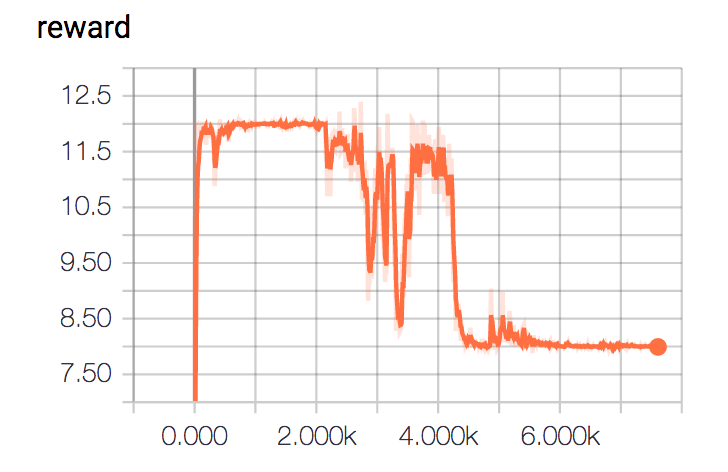
\includegraphics[width=\linewidth]{figures/reinforce-mktrap.png}
  \caption{Learning curve of REINFORCE}
  \label{fig:learning-curve-reinforce-mktrap}
\end{subfigure}
\caption{Learning curve of CMA-ES and REINFORCE for MKTrap}
\label{fig:learning-curve-cma-es-dqn-reinforce-mktrap}
\end{figure}


\section{Genetic Improved Reinforcement Learning (GIRL)}
\label{sec:GIRL}

Inspired by \cite{DBLP:journals/corr/abs-1711-01012}, which applied genetic algorithm on policy based reinforcement learning, we wonder if we can do something similar on value based reinforcement learning. Thus here we have genetic improved reinforcement learning that tries to do Q-learning with some concepts of genetic algorithm. Here each chromosome is an reinforcement learning agent. We first initialize the population consisting of agents with random initialized parameters. Then we do mutation, selection, crossover and so on. The overall algorithm of GIRL is same as \cite{DBLP:journals/corr/abs-1711-01012} as specified in \ref{alg:GIRL}. There are minor difference for each step, and those steps are elaborated in section \ref{sec:GIRL-mutation}, \ref{sec:GIRL-selection}, and \ref{sec:GIRL-crossover}.

\begin{algorithm}
  \caption{Genetic Policy Optimization \label{alg:GIRL}}
  \begin{algorithmic}[1]
    %\Require \fnvar{rl-algorithm} $\mathbb{T}$, \fnvar{Fitness-Fn} $\mathbb{F}$ 
    \Let{\var{population}}{$\pi_1, \dotsc, \pi_m$} \Comment{Initial policies with random parameters}
    
    \Repeat
        \Let{\var{population}}{\fnvar{mutate}(\var{population})}
         
        %\Statex
        
        \Let{\var{parents\_set}}{\fnvar{select}(\var{population}, \fnvar{Fitness-Fn})}
        \Let{\var{children}}{empty set}
        \For{tuple$(\pi_x,\pi_y) \in$ \var{parents\_set}} 
            \Let{$\pi_c$}{\fnvar{crossover}($\pi_x,\pi_y$)}
            \State add $\pi_c$ to \var{children}
        \EndFor
    
        %\Statex
        
        \Let{\var{population}}{\var{children}}
        
    \Until $k$ steps of genetic optimization
   
  \end{algorithmic}
\end{algorithm}


\subsection{GIRL Mutation}
\label{sec:GIRL-mutation}

\cite{DBLP:journals/corr/abs-1711-01012} used policy gradient algorithm for mutation, and here we used Q-learning for mutation. That is, we ran our agent with $\epsilon$-greedy algorithm for episodes and minimized the TD-error. Aside from vanilla Q-learning, improvements such as prioritized experiment replay and double Q-learning are implemented.

\subsection{GIRL Selection}
\label{sec:GIRL-selection}

As \cite{DBLP:journals/corr/abs-1711-01012} did, we selected parents of chromosome rather than selected offspring. For a population of size $n$, their $C^n_2$ pair of parents. We selected parents with highest sum of fitness. And for an agent, here we use the average reward it gets during episodes it runs in the mutation step.

\subsection{GIRL Crossover}
\label{sec:GIRL-crossover}

As \cite{DBLP:journals/corr/abs-1711-01012} did, to generate an offspring, we first composed a hierarchical agent with its parents, and then distill the knowledge from the hierarchical agent to the offspring. In detail, for a pair of parents with Q function $Q_{p0}, Q_{p1}$, we first trained a soft classifier $f$ that predicts which parent is more likely to have seen an observation $s$ using observation of the episodes the parent agents ran in the mutation step as training data. That is, we trained the classifier with data where an observation is labeled with 0 if it was from the experience of parent 0, and is labeled 1 if was from parent 1. Note that the classifier is soft, which implies that $f(s) \in [0, 1]$. So we can compose a hierarchical agent whose Q function $Q_p$ is hierarchical 

\begin{equation}
Q_p(s, a) = (1 - f(s)) Q_{p0}(s, a) + f(s) Q_{p1}(s, a)
\end{equation}

Then we randomly initialized an agent with Q function $Q_c$ as offspring. And again using using observation of the episodes the parent agents ran in the mutation step as training data, we distill knowledge from the hierarchical agent to the offspring by minimizing the loss, namely the difference between $Q_p$ and $Q_c$:

\begin{equation}
L = \sum_{(s, a)} (Q_p(s, a) - Q_c(s, a))^2
\end{equation}

To prevent the distribution of training data and distribution of observation the offspring agent see from mismatching, similar to what \cite{DBLP:journals/corr/abs-1711-01012} did, the technique DAgger \cite{DBLP:journals/jmlr/RossGB11} was also implemented. That is, we used parents' experience as initial training data to train the agent. And then we gather new set of training data from the exploration of the newly trained agent. So we can train the agent with bigger set of data and so on.

\subsection{Experiments}
\label{sec:GIRL-exp}

\subsubsection*{Mountain Car}

In the environment mountain car, the agent need to control the acceleration of the car, and get the flag before timeout (200 steps). The observation seen by the agent is the x-axis coordinate and velocity of the car, and it can decides to accelerate left, right or do nothing. The car cannot climb up the slop directly. So the agent has to control the car back and forth. Note that the reward is negative number of steps taken to get the flag at last step, and -200 if timeout.

% \begin{figure}[h]
% 	\centering
%	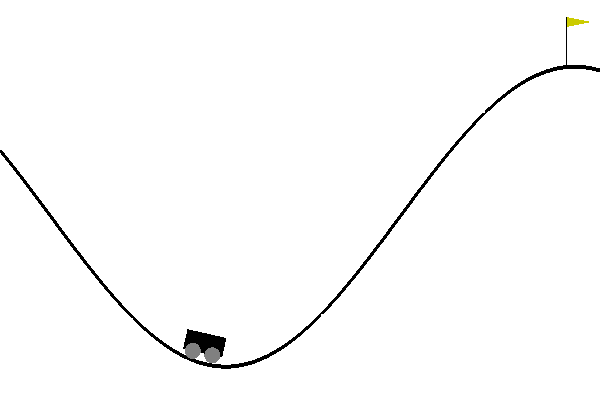
\includegraphics[width=0.5\linewidth]{figures/mountain-car.png}
%  	\caption{Screenshot of environment Mountain Car}
%  	\label{fig:mountain-car}
% \end{figure}

We experiment our GIRL algorithm with population size equals to 4, 5000 steps per generation as the first attempt to see how it works. Good news is that crossover did not destroy pairs of agent disastrously. But unfortunately as shown in figure \ref{fig:learning-curve-girl-mountain-car}, it does not show any advantage compared with original DQN considering 4 times computation power required either.

\begin{figure}[H]
\centering
\begin{subfigure}{.45\textwidth}
  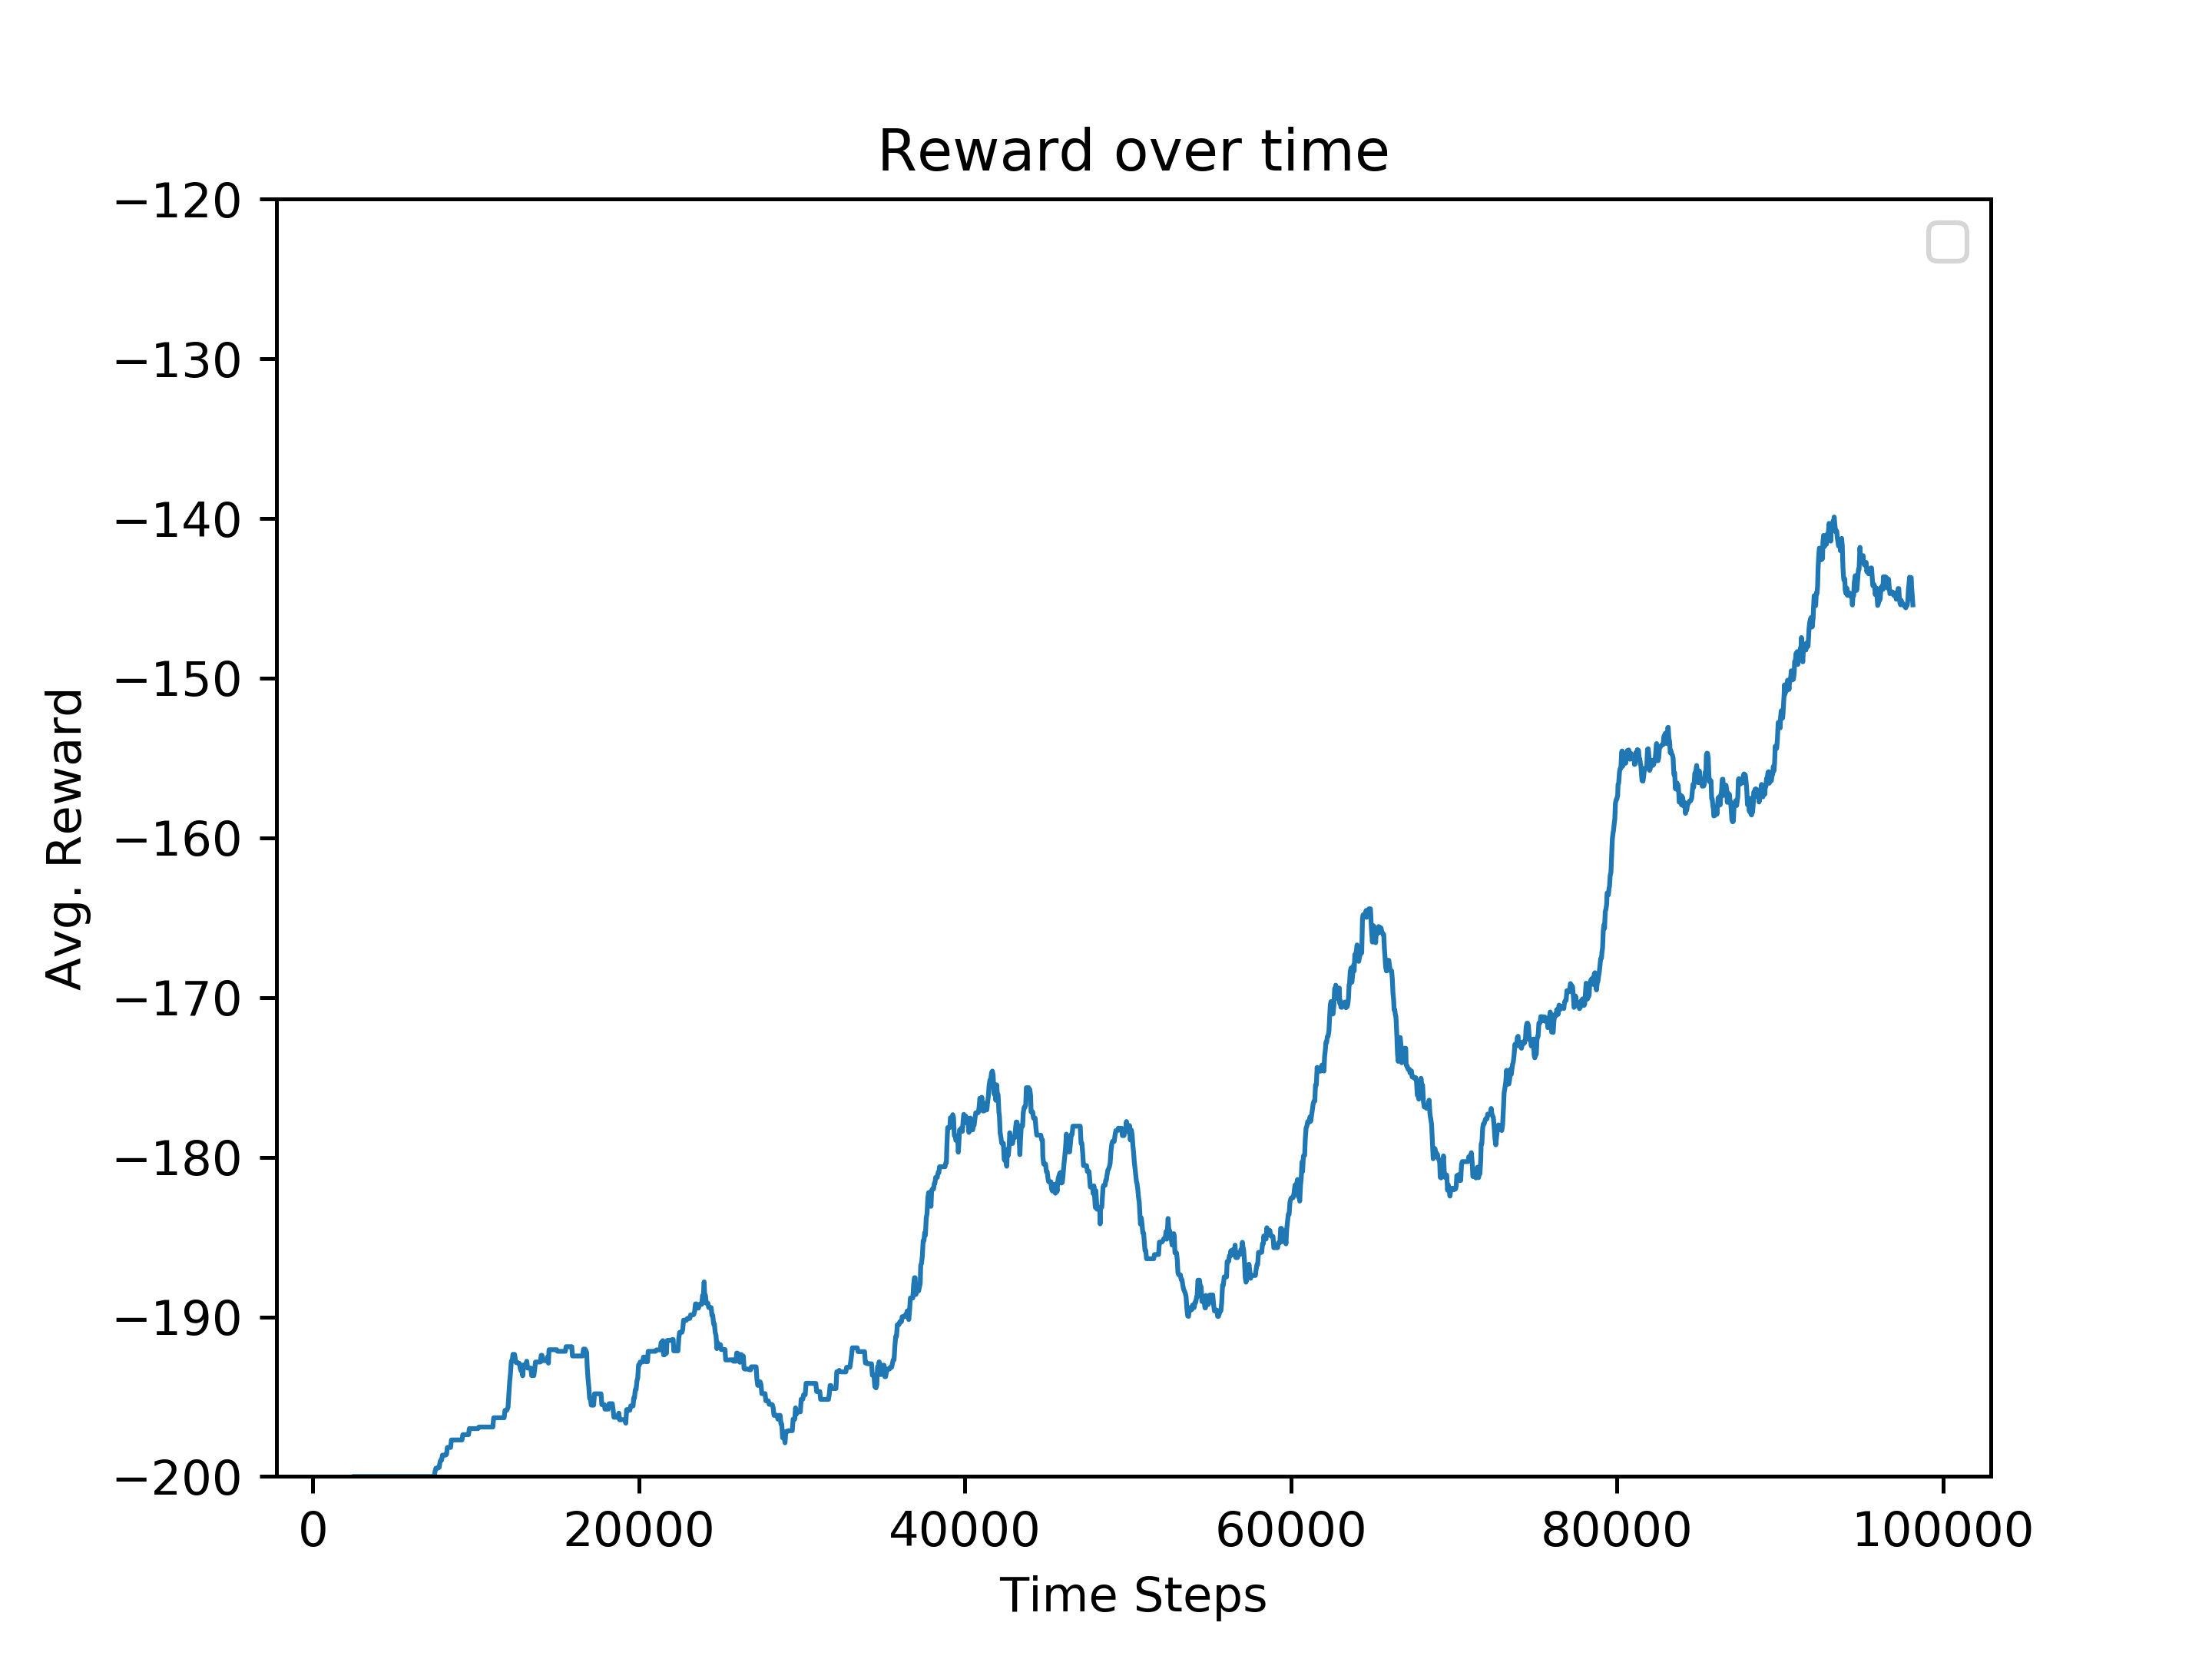
\includegraphics[width=\linewidth]{figures/dqn-mountain-car.png}
  \caption{Learning Curve of DQN}
  \label{fig:learning-curve-dqn-mountain-car}
\end{subfigure}
\begin{subfigure}{.45\textwidth}
  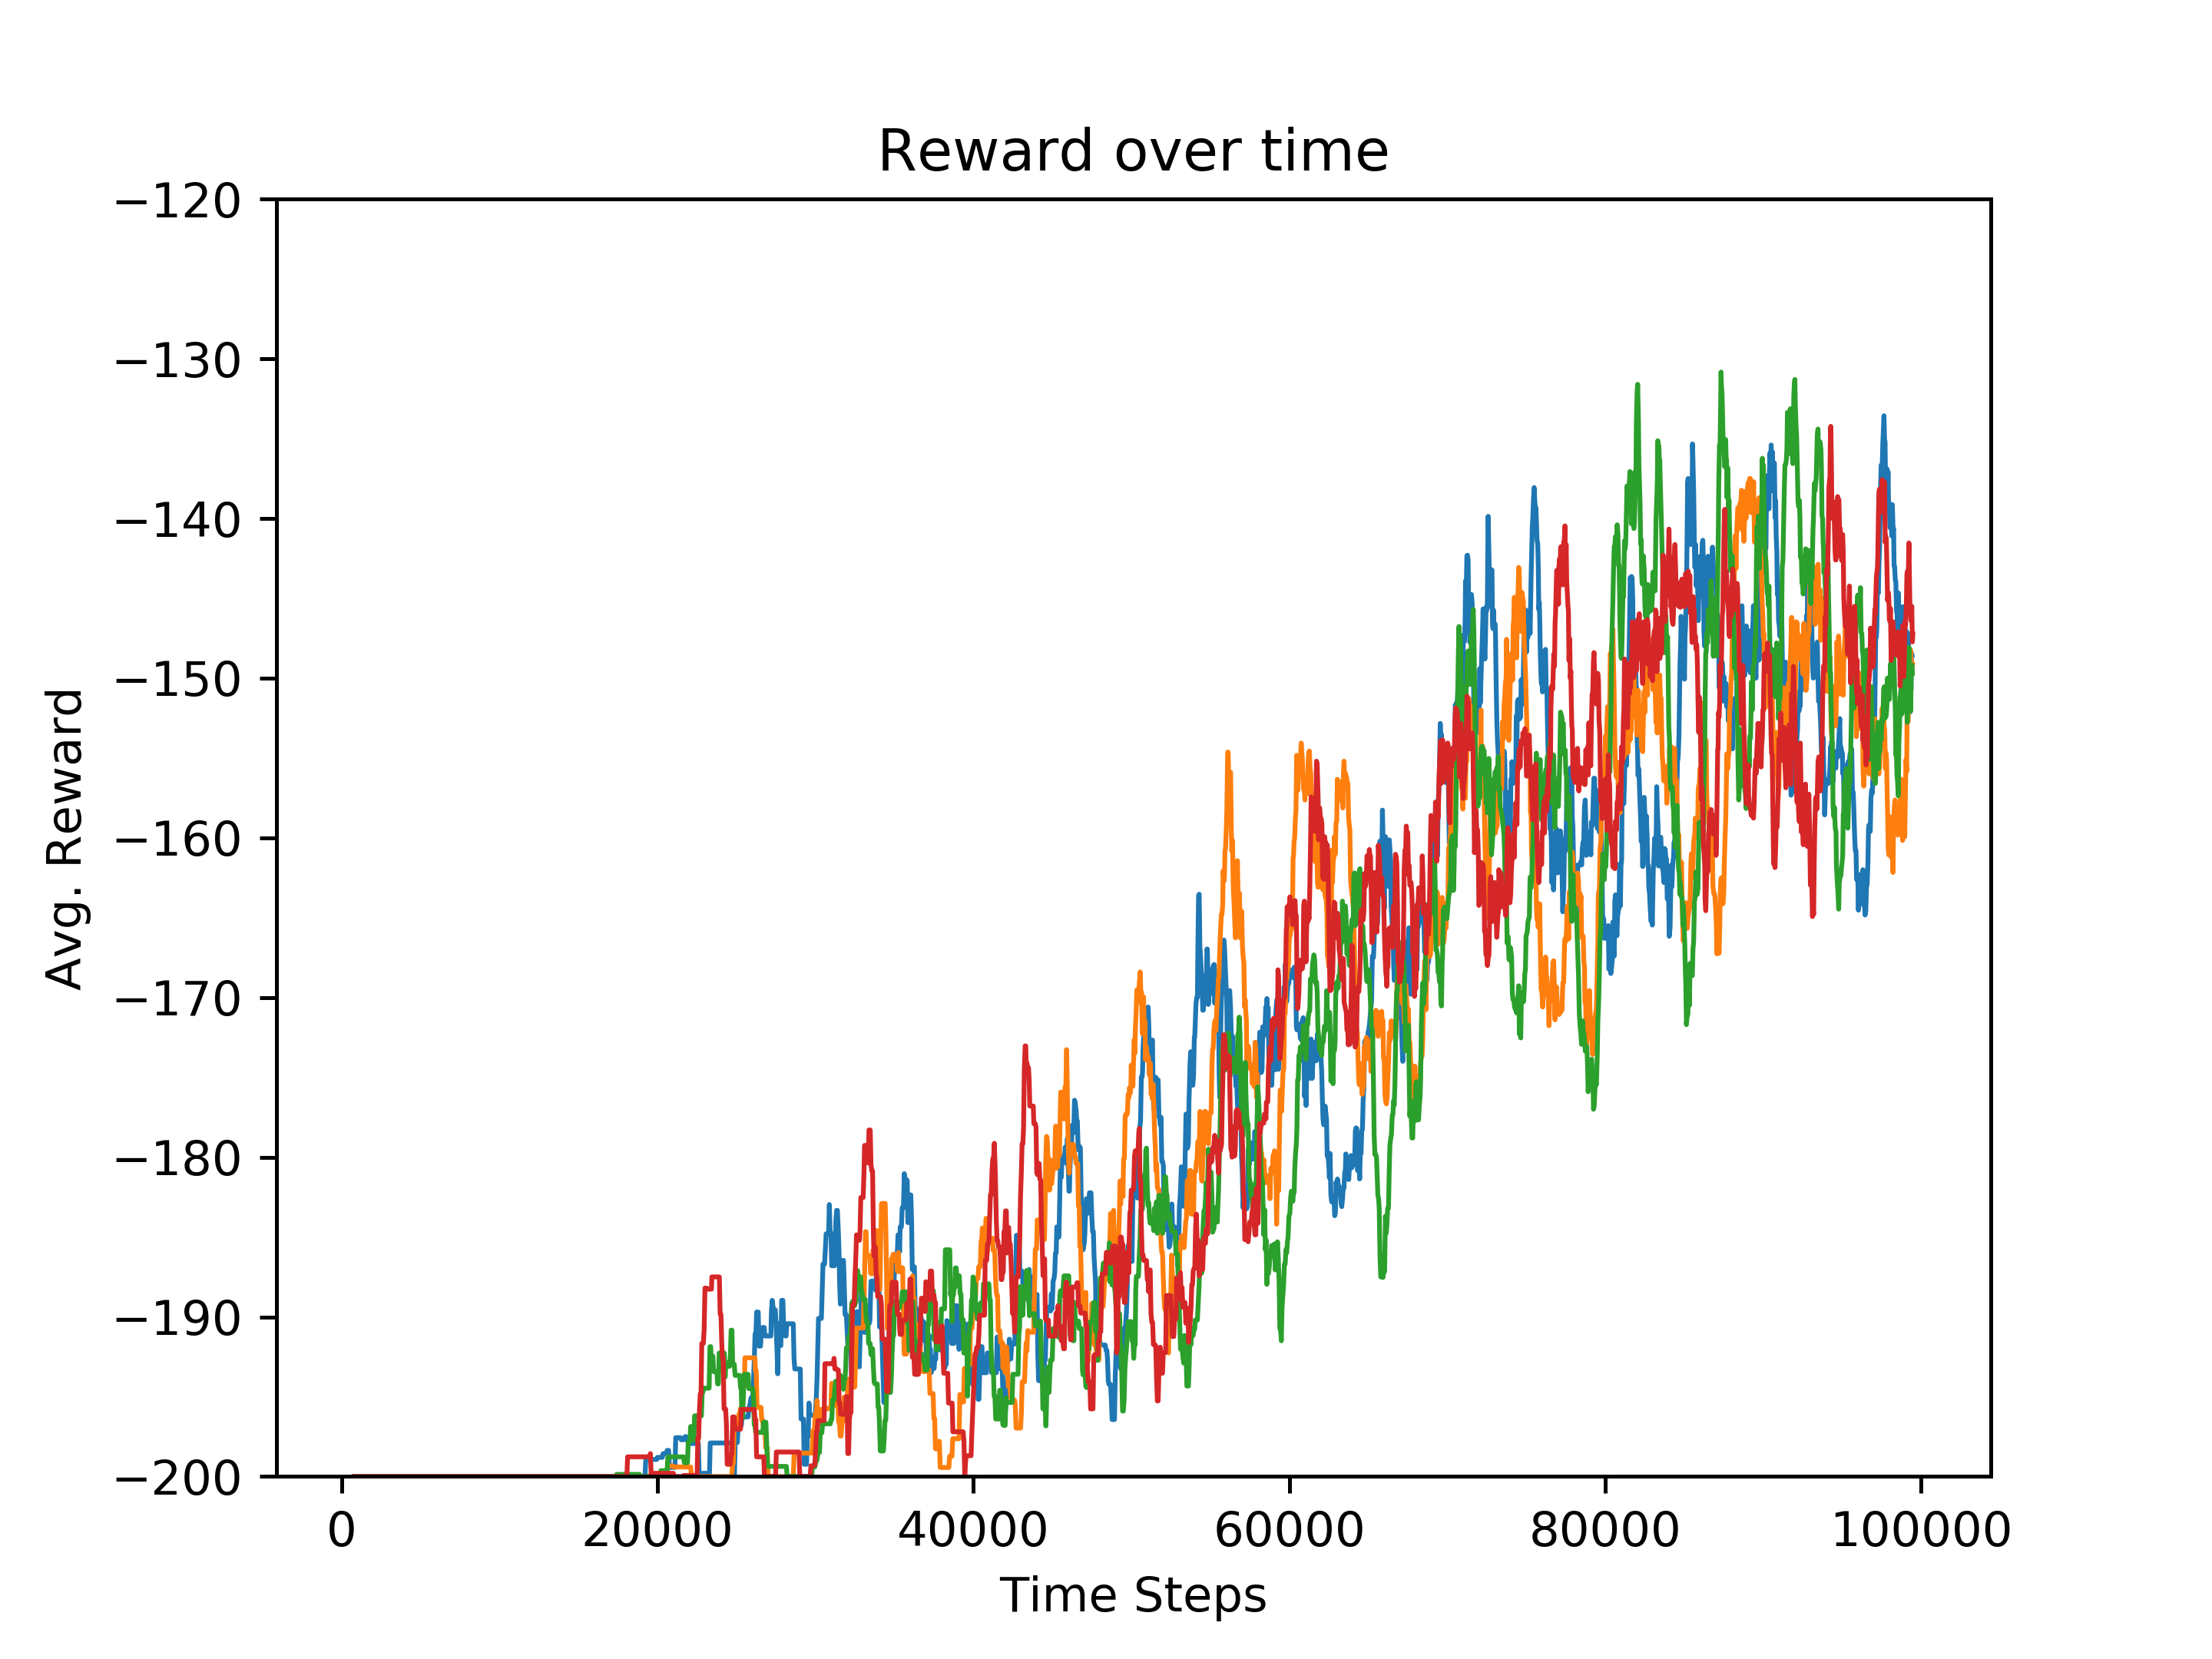
\includegraphics[width=\linewidth]{figures/grl-mountain-car.png}
  \caption{Learning curve of GIRL}
  \label{fig:learning-curve-girl-mountain-car}
\end{subfigure}
\caption{Learning curve of DQN and GIRL for environment mountain car (average reward for 30 episodes.}
\label{fig:learning-curve-dqn-grl-mountain-car}
\end{figure}


\subsubsection*{MK-trap}

We also experiment on MK-trap environment as specified in section \ref{sec:GAvsRL}. Here we use $m=20$, $k=5$. The results are shown in figure \ref{fig:learning-curve-dqn-grl-mktrap} To our surprise, DQN could not solve such problem and cannot not achieve local optimal. And less surprising thing is that GIRL brought no luck.

\begin{figure}[H]
\centering
\begin{subfigure}{.45\textwidth}
  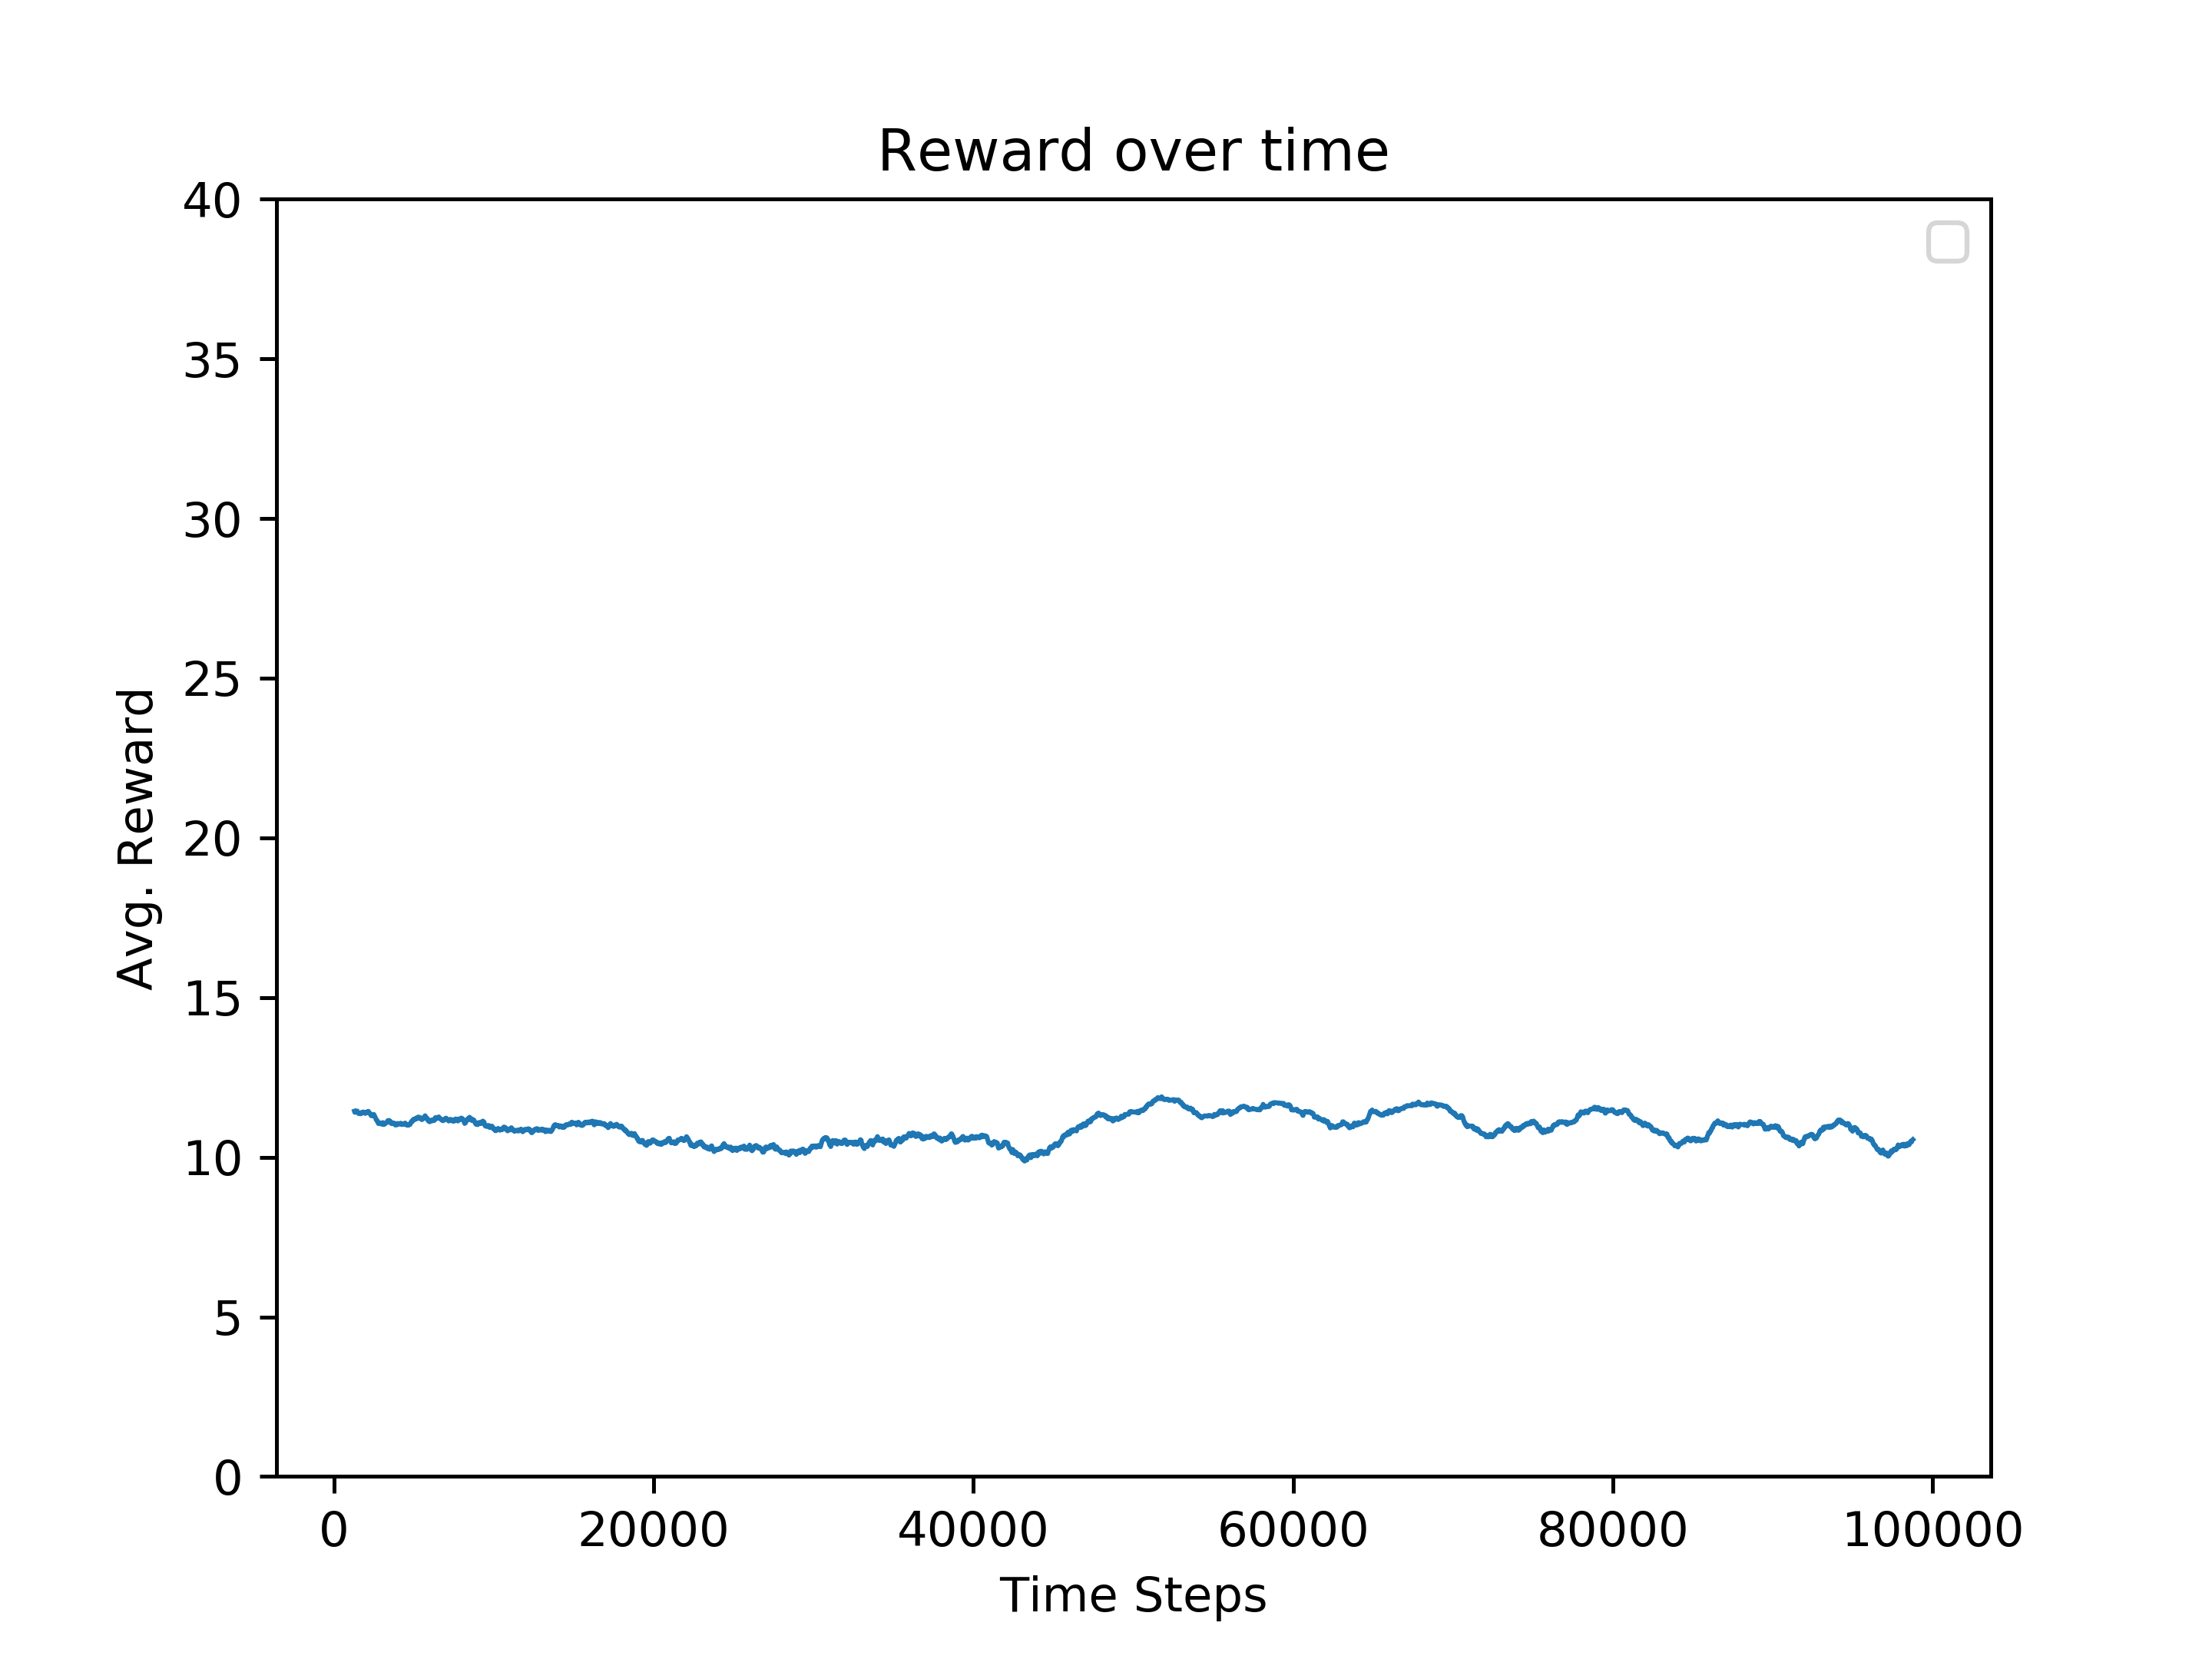
\includegraphics[width=\linewidth]{figures/dqn-mktrap.png}
  \caption{Learning Curve of DQN}
  \label{fig:learning-curve-dqn-mktrap}
\end{subfigure}
\begin{subfigure}{.45\textwidth}
  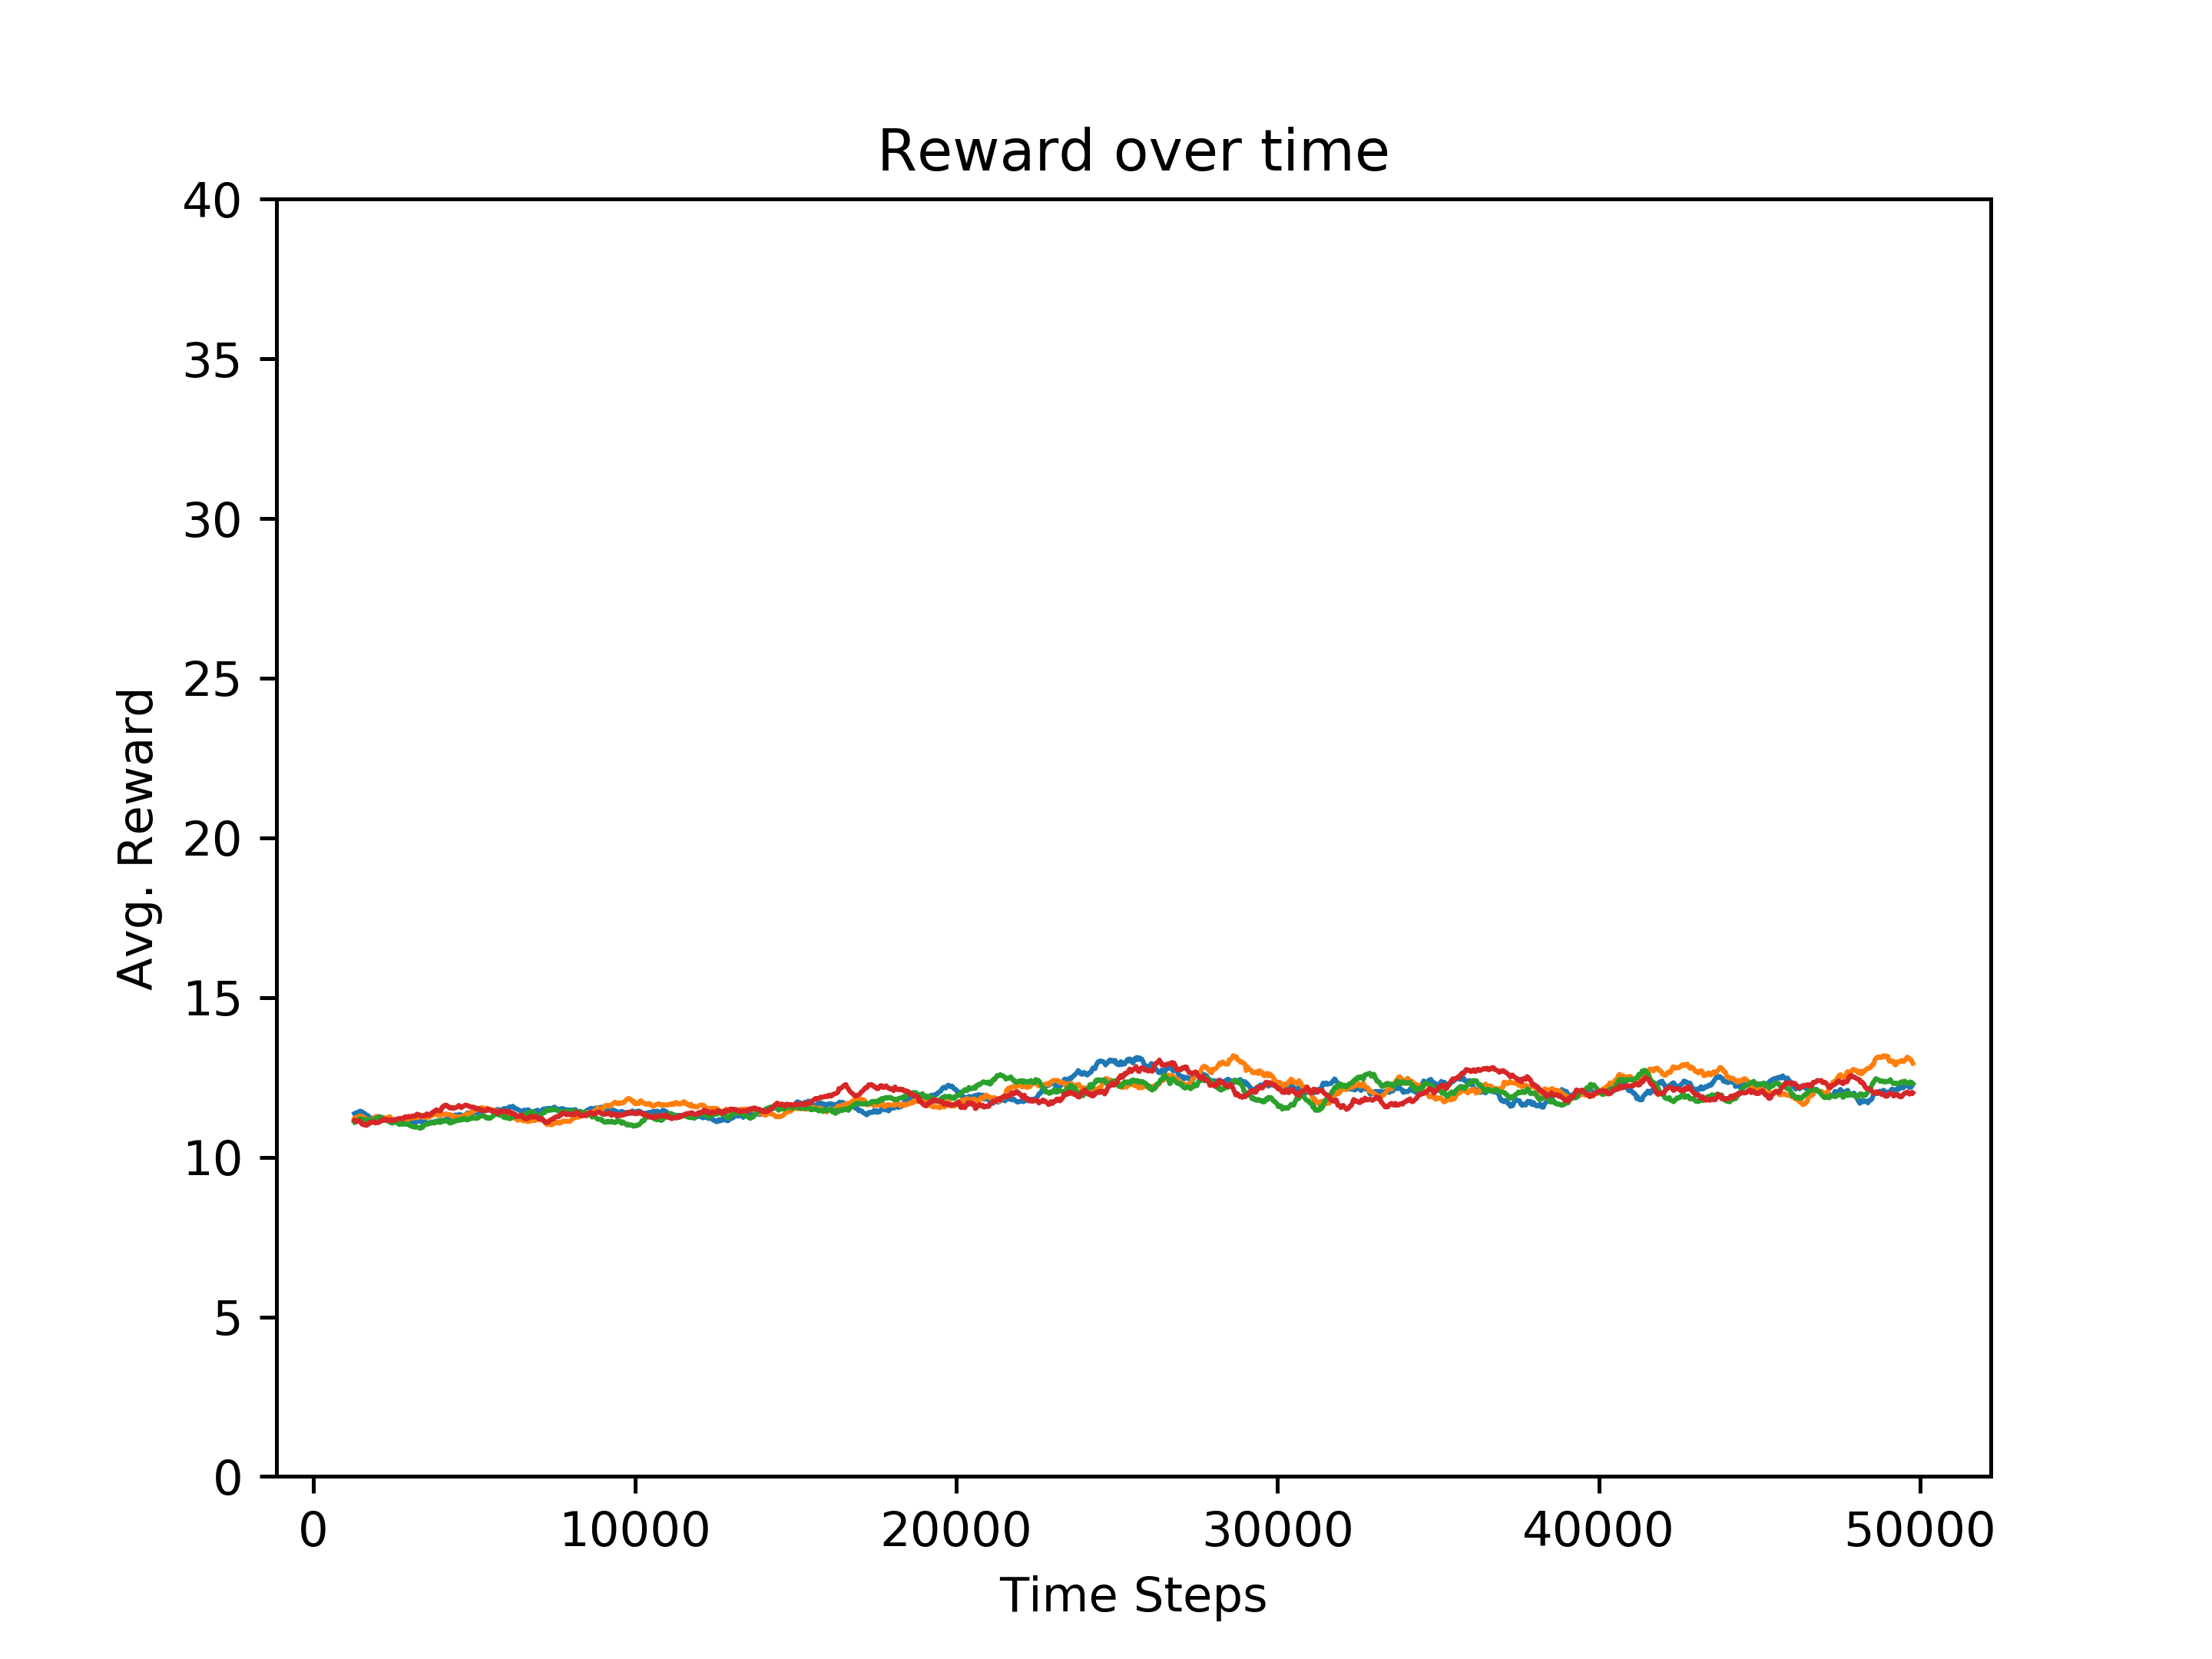
\includegraphics[width=\linewidth]{figures/grl-mktrap.png}
  \caption{Learning curve of GIRL}
  \label{fig:learning-curve-girl-mktrap}
\end{subfigure}
\caption{Learning curve of DQN and GIRL for environment MK-trap (average reward for 30 episodes.}
\label{fig:learning-curve-dqn-grl-mktrap}
\end{figure}


\section{Conclusion}
\label{sec:conclusion}

We have explored and extended recent research on the combination of EC and RL. Using CMA-ES, ES-based RL can have the competitive performance to DQN considering the efficiency of calling fitness function, and bring us more stable training curve and faster training time. And the experiment of combining DQN with GA shows that some more sophisticated design of GA operation may be required to improve value-based reinforcement learning with genetic algorithm. Finally, it is interesting that reinforcement learning cannot solve MK-Trap problem, and it may be a interesting research topic to see why and how to solve it.

\bibliographystyle{alpha}
\bibliography{sample}


\end{document}